\chapter{Prezentacja warstwy użytkowej}
Projekt systemu zarządzania kontem klienta jest zrealizowany jako aplikacja konsolowa. To znaczy że logika jak i działanie programu jest napisane w języku C\#. Program nie posiada dodatkowego interfejsu graficznego a obsługuje się go za pomocą klawiszy z klawiatury. 
Przedstawiam zrzuty ekranu pokazujące działanie programu.

\section{Ekran powitalny}

\begin{figure}[h]
    \centering
    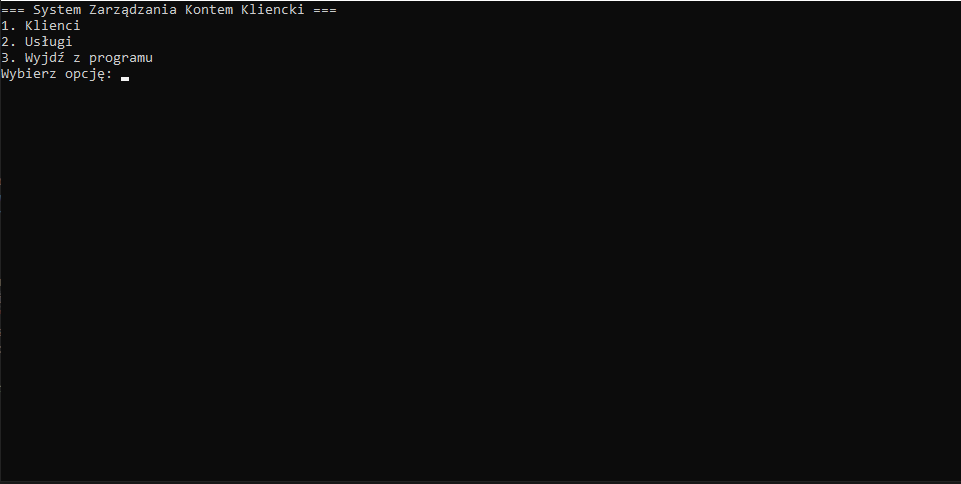
\includegraphics[width=\textwidth]{EkranPow.png}
      \caption{Wybór wyświetlania klienta lub usług}
    \label{fig:example}
\end{figure}

Po uruchomieniu programu w konsoli pokazuje się ekran powitalny z nazwą programu i możliwością przejścia do zakładki klienci lub usługi jest też możliwość zakończenia programu. 

\newpage

\section{Zarządzanie Klientami}

\begin{figure}[h]
    \centering
    \includegraphics[width=\textwidth]{ZarządzanieKlientami.png}
      \caption{Wybór operacji na koncie klienta}
    \label{fig:example}
\end{figure}

Po przejściu do zakładki klientckiej pokazuje się ekran powitalny z menu wyboru odpowiedniej operacji. 

\subsection{Wyświetlanie informacji o klientach}
\begin{figure}[h]
    \centering
    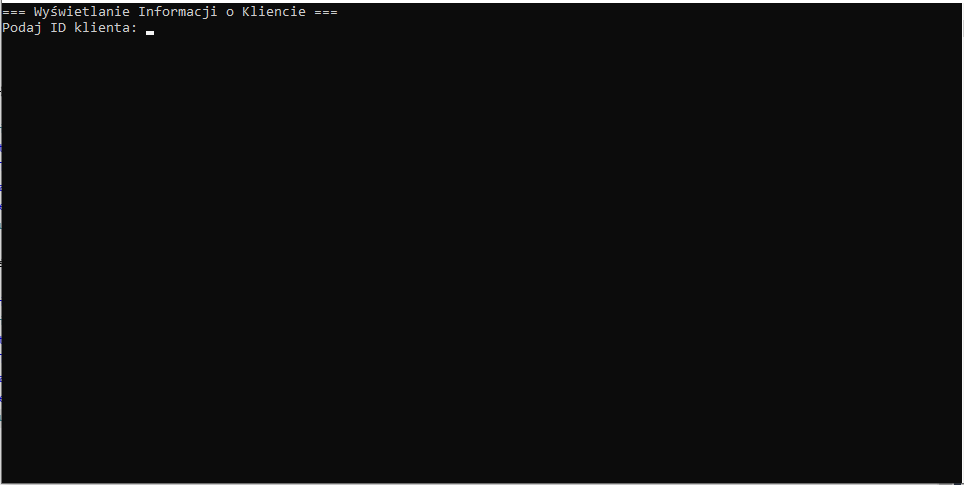
\includegraphics[width=\textwidth]{WysInf.png}
      \caption{Wprowadzanie ID klienta}
    \label{fig:example}
\end{figure}

Wybierając opcję wyświetlenia informacji o kliencie program poprosi o podanie ID klienta którego chcemy wyświetlić.

\subsubsection{Wybór odpowiedniego klienta}
\begin{figure}[h]
    \centering
    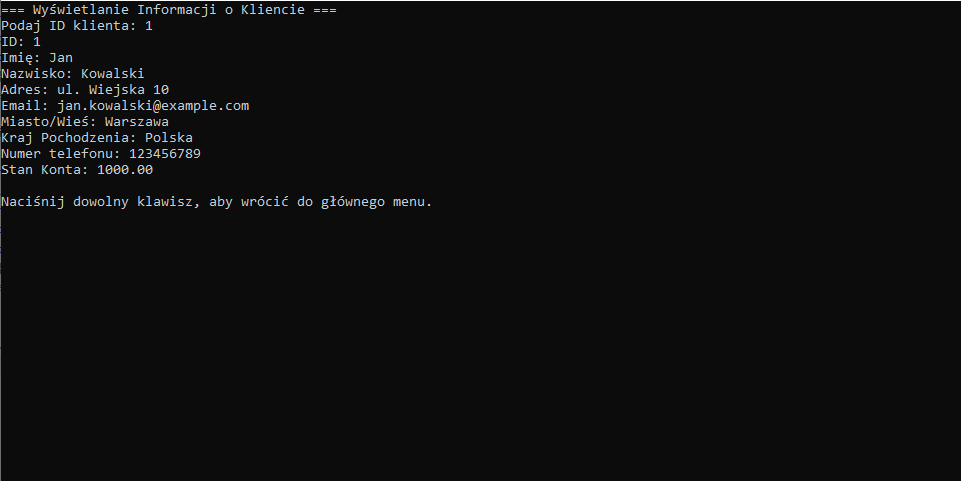
\includegraphics[width=\textwidth]{WysInf1.png}
      \caption{Przedstawienie danych klienta}
    \label{fig:example}
\end{figure}

Po wybraniu odpowiedniego klienta zostaną wyświetlone wszystkie dane pobrane z bazy danych. 

\subsubsection{Wybór klienta którego nie ma w systemie}
\begin{figure}[h]
    \centering
    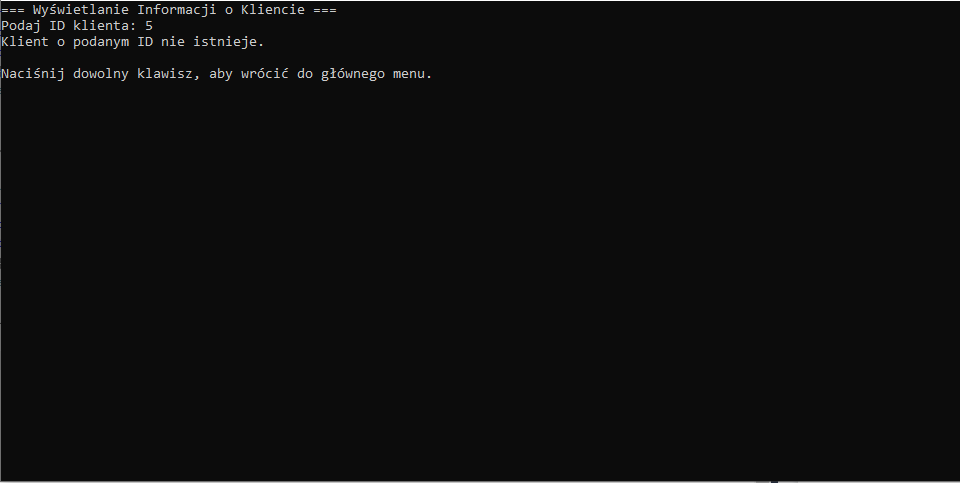
\includegraphics[width=\textwidth]{WysInfBrak.png}
      \caption{Brak klienta o wybranym ID}
    \label{fig:example}
\end{figure}

Jeśli zostanie wybrany klient którego nie ma w systemie program zwróci odpowiednią informację i będziemy mieć możliwość wyszukać ponownie klienta. 

\newpage

\subsection{Dodawanie klienta}


\begin{figure}[h]
    \centering
    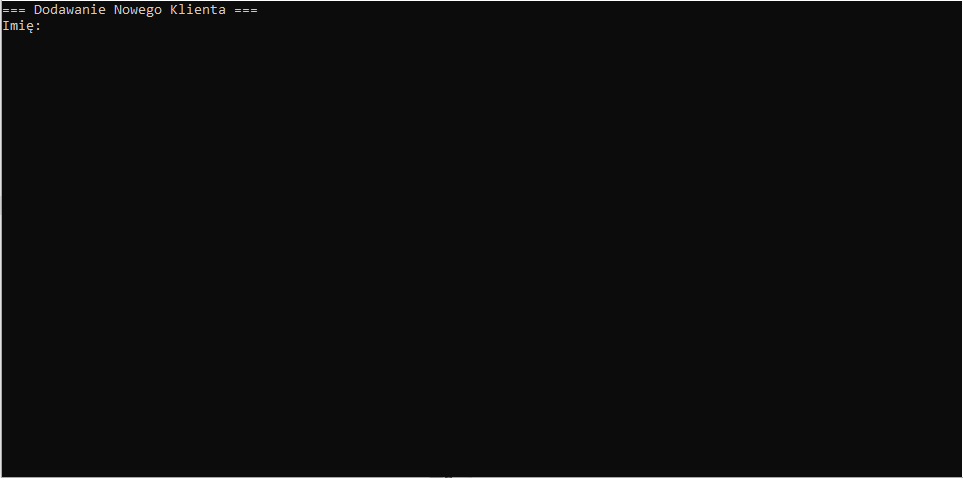
\includegraphics[width=\textwidth]{DodawanieKlienta.png}
      \caption{Możliwość dodania nowego klienta}
    \label{fig:example}
\end{figure}

Wybierając opcje dodania klienta system poprosi nas o wpisanie wszystkich wartości potrzebnych żeby dodać klienta do systemu. 

\subsubsection{Dodanie klienta dane wprowadzone poprawnie}
\begin{figure}[h]
    \centering
    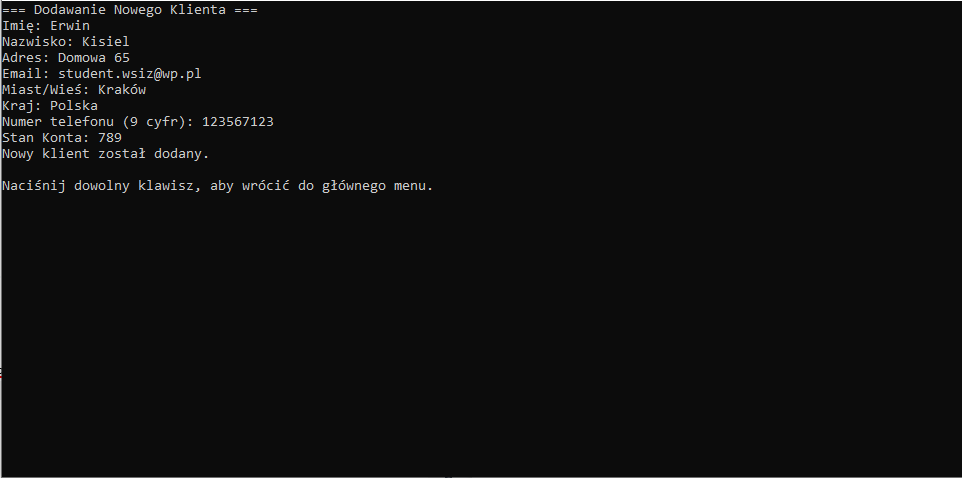
\includegraphics[width=\textwidth]{DodawanieKlientaPop.png}
      \caption{Dodanie klienta do systemu}
    \label{fig:example}
\end{figure}

Po wpisaniu poprawnych danych klient zostanie dodany do systemu automatycznie zostanie mu nadany kolejny numer id.
\newpage
\subsubsection{Dodanie klienta dane wprowadzone błędnie}
\begin{figure}[h]
    \centering
    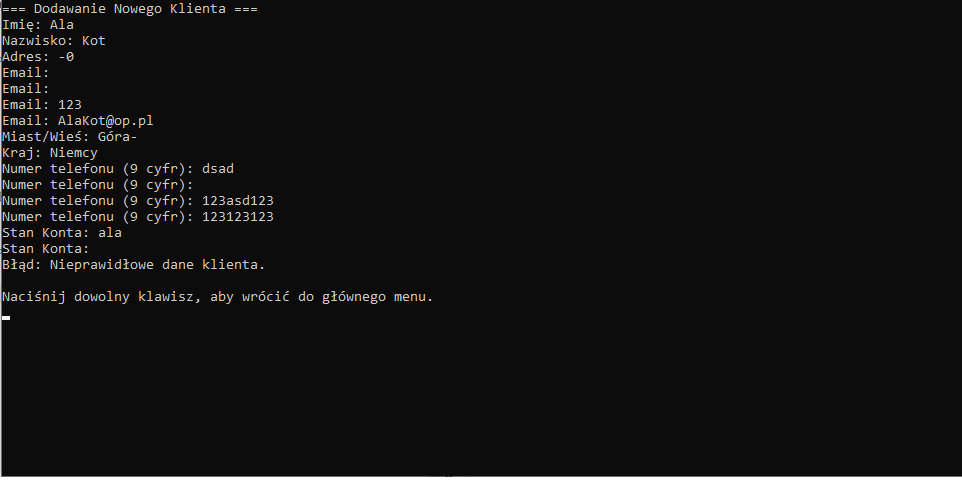
\includegraphics[width=\textwidth]{DodawanieKlientaBle.png}
      \caption{Błąd dodania klienta do systemu}
    \label{fig:example}
\end{figure}

Dodając klienta możemy pomylić się w wielu miejscach dlatego program pozwoli nam przejść dalej lub ponowi możliwość wpisania danej wartości jeśli w miejsce wymagane zostanie wpisana pusta wartość program przejdzie dalej niestety dodawanie zakończy sie niepowodzeniem i trzeba będzie powtórzyć jednak jeśli ktoś się pomyli podczas wpisywania numeru telefonu wpisze więcej cyfr lub doda niedozwolony znak program poprosi go o ponowne wpisanie danej wartości. 

\subsection{Aktualizowanie danych klienta}

\begin{figure}[h]
    \centering
    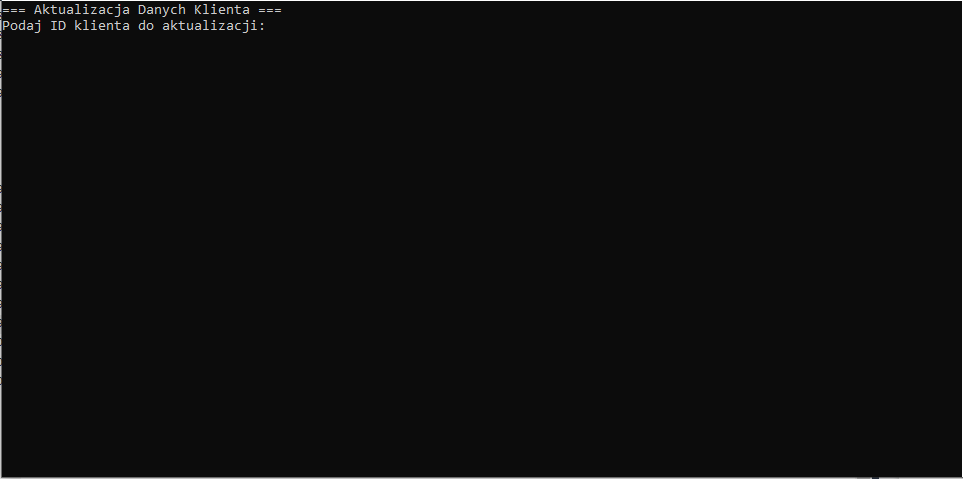
\includegraphics[width=\textwidth]{AktualizacjaDanych.png}
      \caption{Możliwość aktualizacji błędnych danych}
    \label{fig:example}
\end{figure}

Wybierając opcję aktualizacji danych kliencie program poprosi o podanie ID klienta którego chcemy wyświetlić.

\subsubsection{Aktualizowanie danych klienta dane wprowadzone poprawnie}

\begin{figure}[h]
    \centering
    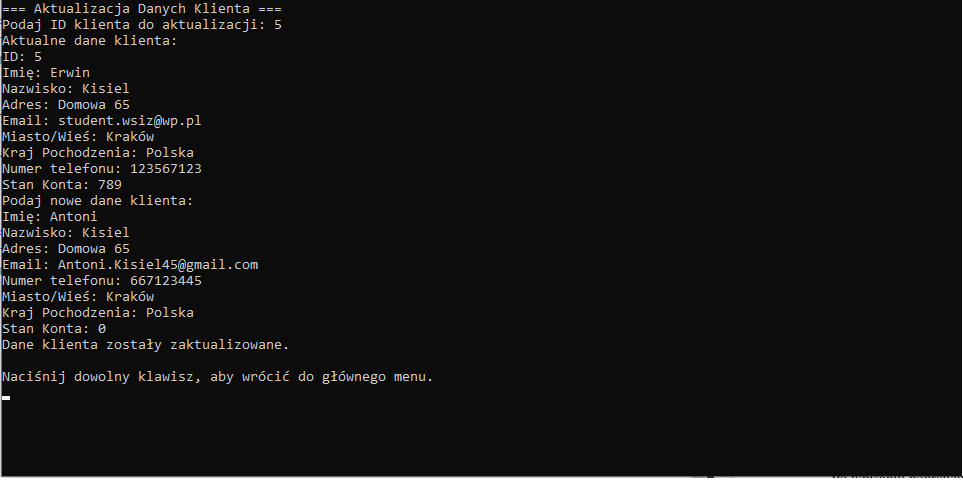
\includegraphics[width=\textwidth]{AktualizacjaDanychPop.png}
      \caption{Możliwość aktualizacji błędnych danych}
    \label{fig:example}
\end{figure}

Po wybraniu klienta którego dane chcemy zaktualizować dostajemy podgląd na dane jakie aktualnie posiada klient i na ich podstawie może wpisać poprawione informacje. 

\subsubsection{Aktualizowanie danych klienta dane wprowadzone błędnie}

\begin{figure}[h]
    \centering
    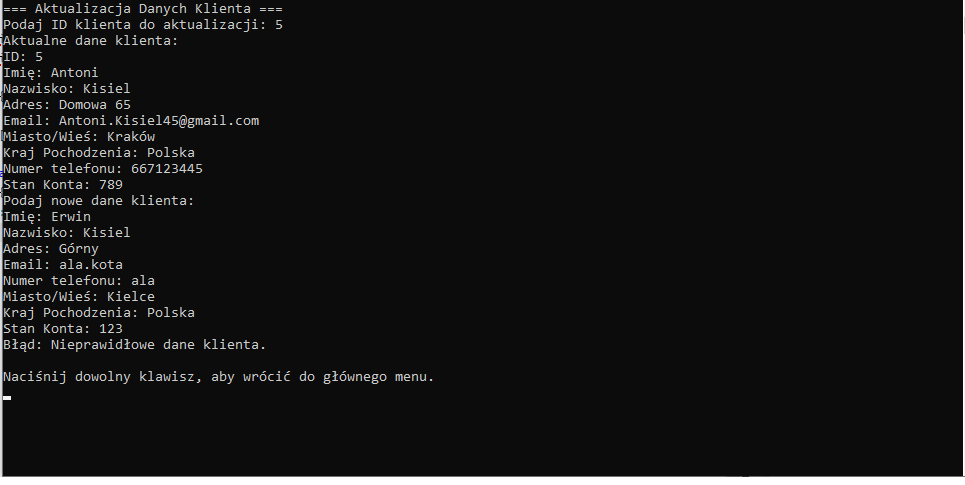
\includegraphics[width=\textwidth]{AktualizacjaDanychNeg.png}
      \caption{Możliwość aktualizacji błędnych danych}
    \label{fig:example}
\end{figure}

Program wykrywa dane które się nie zgadzają nie przedstawia błędu nie prosi też o wpisanie ponownie danej wartości dopiero pod koniec przekazuje że dane nie zostały zaktualizowane i pokazuje błąd. Użytkownik musi od nowa aktualizować dane tym razem bez błędu. 

\subsubsection{Weryfikacja zaktualizowanych danych}

\begin{figure}[h]
    \centering
    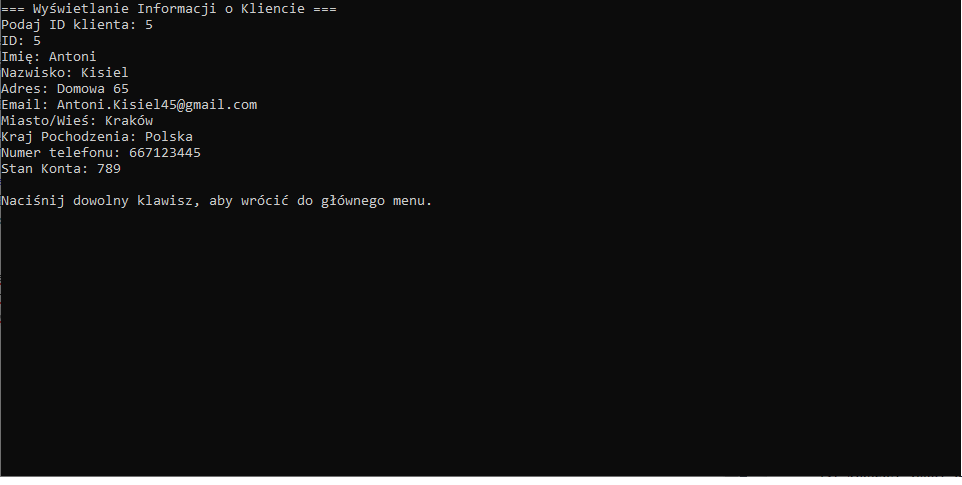
\includegraphics[width=\textwidth]{AktualizacjaDanychWer.png}
      \caption{Weryfikacja danych klienta}
    \label{fig:example}
\end{figure}

Dane klienta zostały zaktualizowane podczas poprawnego wprowadzenia wartości do systemu za to drugim razem po wykonaniu błędu system już nie zmienił wartości. 

\subsection{Usuwanie danych klienta}

\begin{figure}[h]
    \centering
    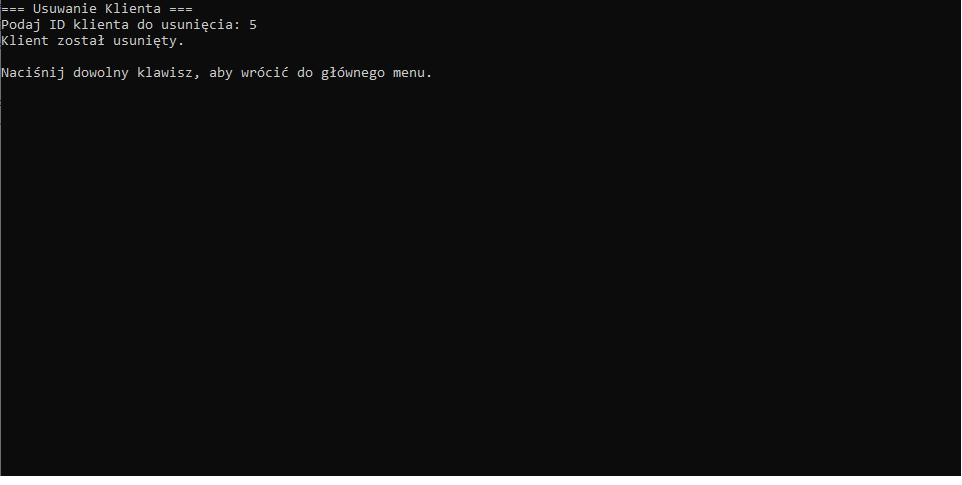
\includegraphics[width=\textwidth]{UsuwanieKlienta.png}
      \caption{Możliwość usuwania klienta z systemu}
    \label{fig:example}
\end{figure}

Wybierając opcję usuwania informacji o kliencie program poprosi o podanie ID klienta którego chcemy usunąć.

\subsubsection{Weryfikacja usuniętych danych klienta}
\begin{figure}[h]
    \centering
    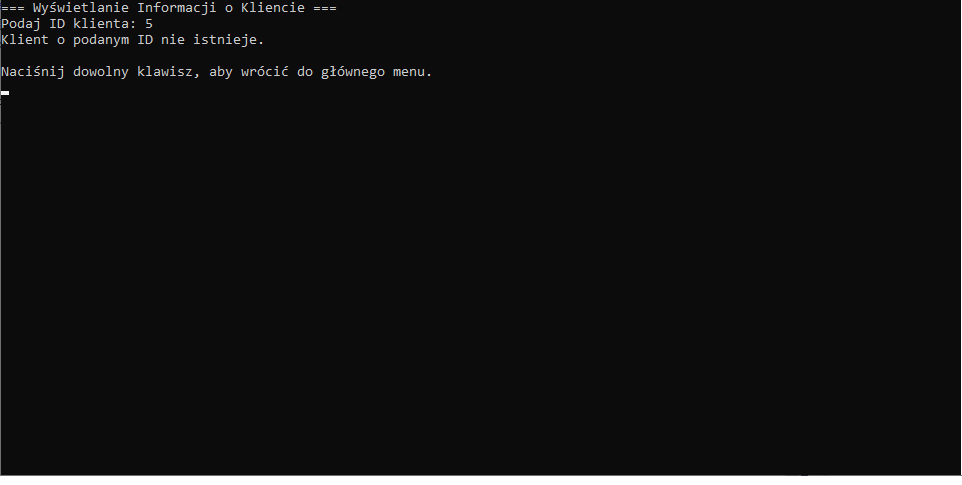
\includegraphics[width=\textwidth]{PotwierdzenieUsu.png}
      \caption{Potwierdzenie usunięcia}
    \label{fig:example}
\end{figure}

\section{Zarządzanie Usługami}

\begin{figure}[h]
    \centering
    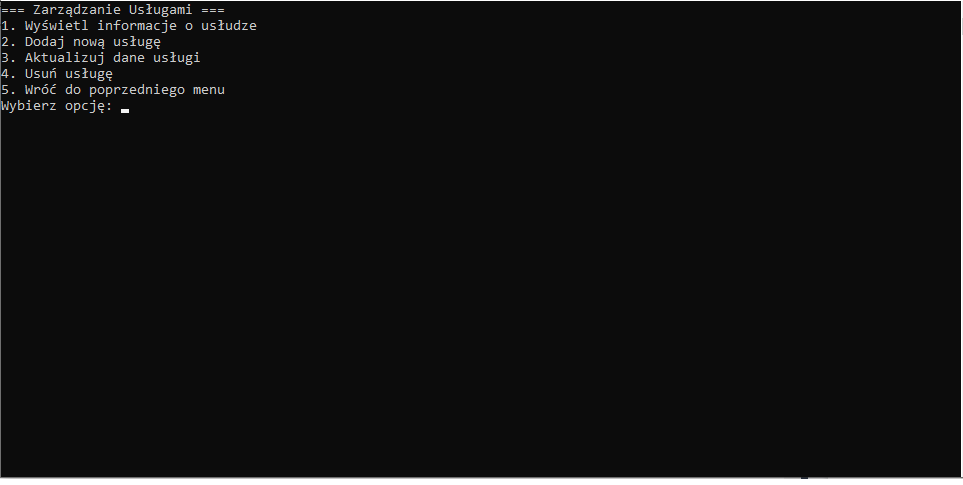
\includegraphics[width=\textwidth]{ZarzadUslug.png}
      \caption{Prezentacja opcji w usługach}
    \label{fig:example}
\end{figure}
Po przejściu do zakładki z usługami pokazuje się ekran powitalny z menu wyboru odpowiedniej operacji. 

\subsection{Wyświetlanie informacji o usługach}

\begin{figure}[h]
    \centering
    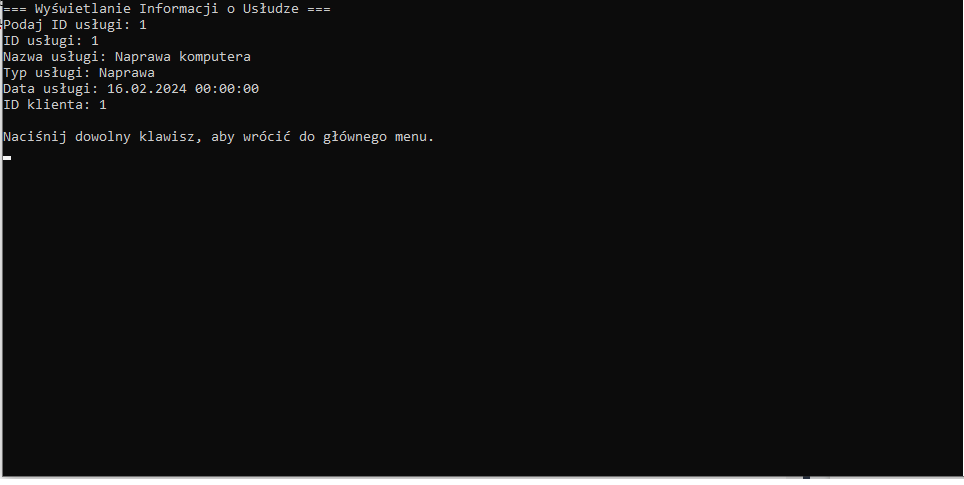
\includegraphics[width=\textwidth]{WysInfUslug.png}
      \caption{Przedstawienie danych usługi}
    \label{fig:example}
\end{figure}

Wybierając opcję wyświetlenia informacji o usługacg program poprosi o podanie ID klienta którego chcemy wyświetlić.

\subsection{Dodawanie usług}
\begin{figure}[h]
    \centering
    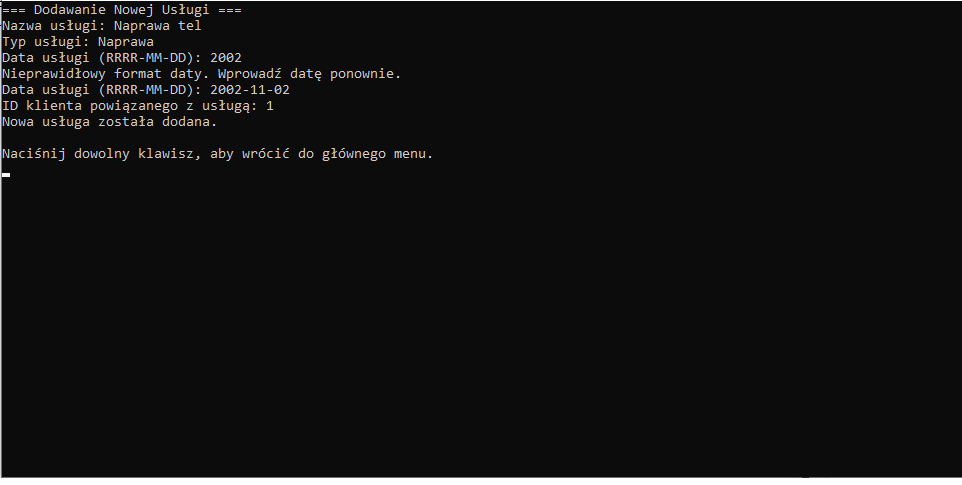
\includegraphics[width=\textwidth]{DodawanieUslug.png}
      \caption{Dodanie usługi do systemu}
    \label{fig:example}
\end{figure}

\newpage
Wybierając opcje dodania usługi system poprosi nas o wpisanie wszystkich potrzebnych danych.

\subsection{Aktualizacja danych w usługach}
\begin{figure}[h]
    \centering
    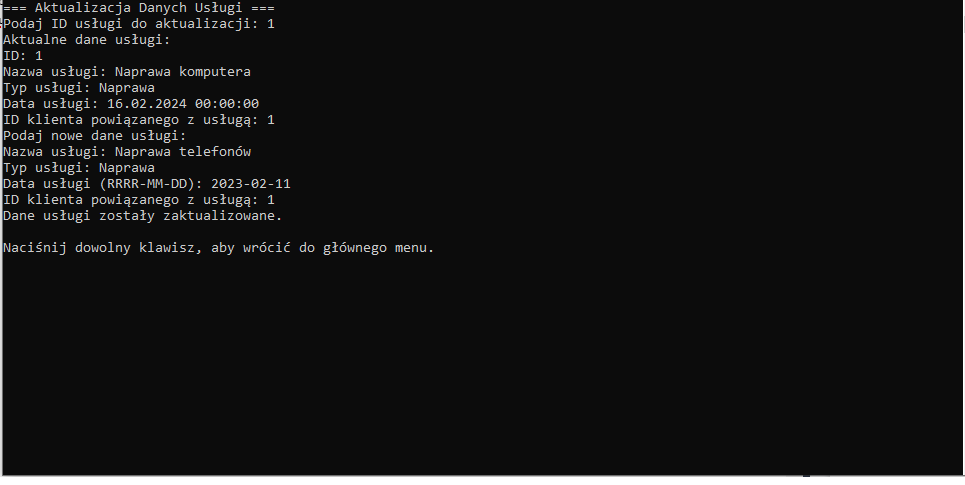
\includegraphics[width=\textwidth]{AktualizacjaDanychUslug.png}
      \caption{Zaktualizowanie danych o usłudze}
    \label{fig:example}
\end{figure}

Po wybraniu usługi którą chcemy zaktualizować dostajemy podgląd i na jego podstawie może wpisać poprawione informacje. 



\subsection{Usuwanie usług}
\begin{figure}[h]
    \centering
    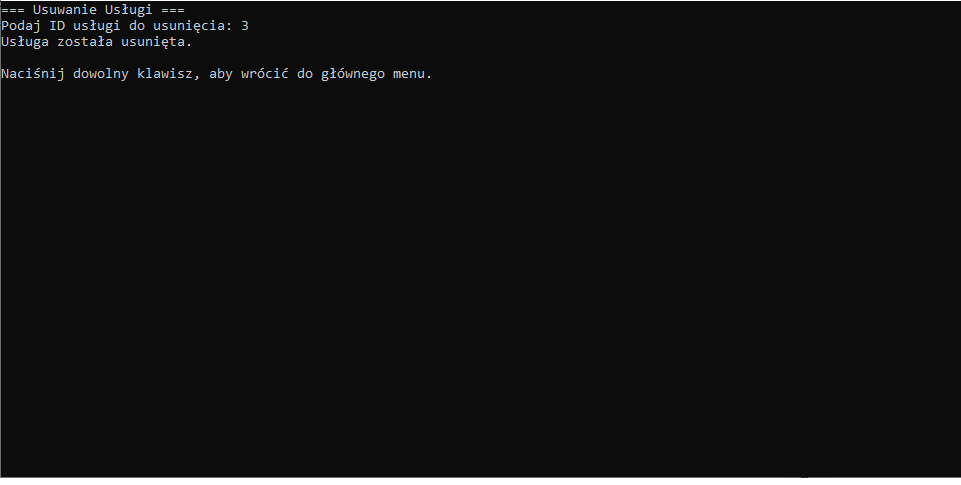
\includegraphics[width=\textwidth]{UsuwanieUslug.png}
      \caption{Usunięcie usługi}
    \label{fig:example}
\end{figure}

Wybierając opcję usuwania informacji o usłudze program poprosi o podanie ID dzięki niemu może odnaleźć usługę do usunięcia.